\begin{figure*}[htb]
  \centering
  \begin{subfigure}[t]{0.32\textwidth}
    \centering
    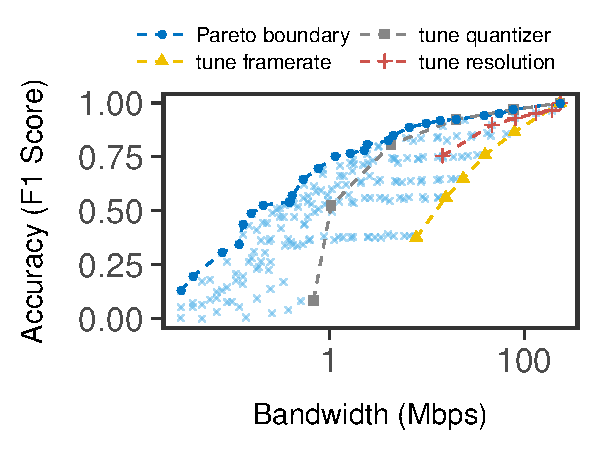
\includegraphics[width=\textwidth]{figures/profile-darknet.pdf}
    \caption{Augmented Reality (AR)}
    \label{fig:ar-profile}
  \end{subfigure}
  \hfill
  \begin{subfigure}[t]{0.32\textwidth}
    \centering
    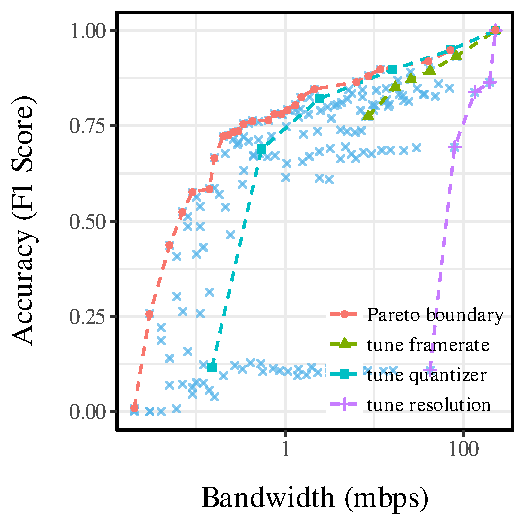
\includegraphics[width=\textwidth]{figures/profile-mot.pdf}
    \caption{Pedestrian Detection (PD)}
    \label{fig:pd-profile}
  \end{subfigure}
  \hfill
  \begin{subfigure}[t]{0.32\textwidth}
    \centering
    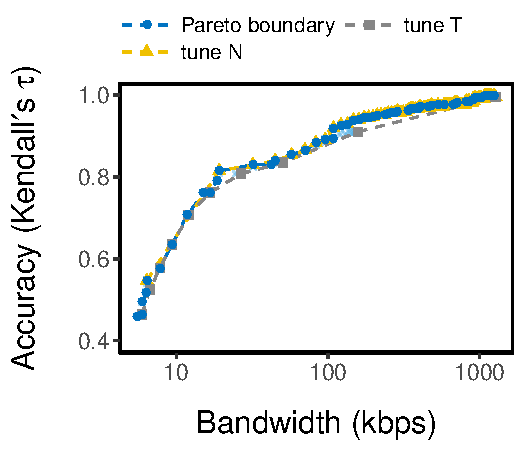
\includegraphics[width=\textwidth]{figures/profile-topk.pdf}
    \caption{Top-K (TK)}
    \label{fig:tk-profile}
  \end{subfigure}
  \caption{Application profiles of three applications. Each cross point is one
    configuration $c$'s performance $(B(c), A(c))$. All figures show the Pareto
    boundary as well as the performance if only tuning one dimension. Note the
    x-axis is in log scale.}
  \label{fig:all-profiles}
\end{figure*}

\section{Evaluation}
\label{sec:evaluation}

In this section, we show the evaluations of \sysname{}, summarizing the results
as follows.

\begin{itemize}[itemsep=0pt, topsep=3pt]
\item[\autoref{sec:application-profiles}] \sysname{} generates Pareto-optimal
  profiles across multiple dimensions with precision
  (\autoref{fig:all-profiles}).
\item[\autoref{sec:online-profiling}] Our parallel and sampling techniques
  speeds up offline and online profiling (\autoref{fig:parallel},
  \autoref{fig:online-tricks}).
\item[\autoref{sec:runtime-adaptation}] At runtime, \sysname{} achieves
  sub-second latency and nominal accuracy drop for all applications
  (\autoref{fig:ar-runtime}, \autoref{fig:pd-tk}) and across various network
  conditions (\autoref{fig:ar-rtt}).
\item[\autoref{sec:multi-task-alloc}] \sysname{} profiles allow different
  resource allocations: resource fairness and utility fairness
  (\autoref{fig:multitask}).
\end{itemize}

\subsection{Application Profiles}
\label{sec:application-profiles}

We run offline profiling using the training dataset described
in~\autoref{tab:apps} and show the learned profiles in
\autoref{fig:all-profiles}. In each figure, the cross dots represent the
bandwidth demand and application accuracy for one configuration. We highlight
the Pareto-optimal boundary $\mathbb{P}$ with blue dashed lines. To understand
each dimension's impact on the degradation, we highlight configurations from
tuning only \textit{one} dimension. From these profiles, we make the following
observations:

\para{Large bandwidth variation.} For all three applications, The bandwidth
requirements of all three applications have two to three orders of magnitude of
difference (note the x-axis is in log scale). For AR and PD, the most expensive
configuration transmits videos at 1920x1080, 30 FPS and 0 quantization; it
consumes \SI{230}{Mbps}. In contrast to the large bandwidth variation, there is
a smaller variation in accuracy. In PD, for example, even after the bandwidth
reduces to \SI{1}{Mbps} (less than 1\% of the maximum), the accuracy is still
above 75\%. The large variation allows \sysname{} to operate at a high accuracy
configuration even under severe network deterioration.

\para{Distinct effects by each dimension.} Comparing dashed lines in each
profile, we see that the Pareto-optimal configurations are only achievable when
multiple knobs are in effect. Tuning only one dimension often leads to
sub-optimal performance. Within a single profile, the difference between tuning
individual dimensions is evident. For PD, tuning resolution (the red line) leads
to a quicker accuracy drop than tuning frame rate (the yellow line). Comparing
AR and PD, the same dimension has different impact. Tuning resolution is less
harmful in AR than PD; while tuning frame rate hurts AR more than PD\@. This
echoes our initial observation in~\autoref{subsec:motivation} that
application-specific optimizations do not generalize.

% \para{Quantification with precision}. The generated profiles are actionable
% configurations that control the knobs with precision. For example, if PD
% transmits video at 1920x1080 resolution, \(10~\text{FPS}\) and a quantization
% of 20, it will consume 11.7 mbps of bandwidth, achieving roughly 90\%
% accuracy. This saves developers from laboriously analyzing their application
% to compute manual policies.

\subsection{Profiling Efficiency \& Online Profiling}
\label{sec:online-profiling}

This section focuses on the AR application as a case study; our profiling
techniques---parallelism and sampling---do not make assumptions about the
application; therefore, the evaluation results can be generalized to other
applications.

In AR, there are 216 different configurations: 6 resolutions, 6 frame rates and
6 quantization levels. AR uses YOLO~\cite{redmon2016yolo9000}, a neural network
model for object detection. It takes roughly \SI{30}{\ms} to process one frame
on GeForce\textregistered\space GTX 970.\footnote{YOLO resizes images to fixed
  416$\times$416 resolutions as required by the neural network. Evaluating
  images with different resolutions takes similar time.}  But different
configurations require different times for processing. For example, a
\(10~\text{FPS}\) video has 1/3 of the frames to process in comparison to a
\(30~\text{FPS}\) video.  In our experiment, to evaluate all 216 configurations,
it takes 52 seconds for 1 second worth of data. We denote such overhead as
52X\@. \hyperref[sec:automatic-profiling]{Section 3.2} discusses parallel and
sampling techniques to improve the profiling efficiency; we present their
evaluations as follows.

\begin{figure}
  \centering
  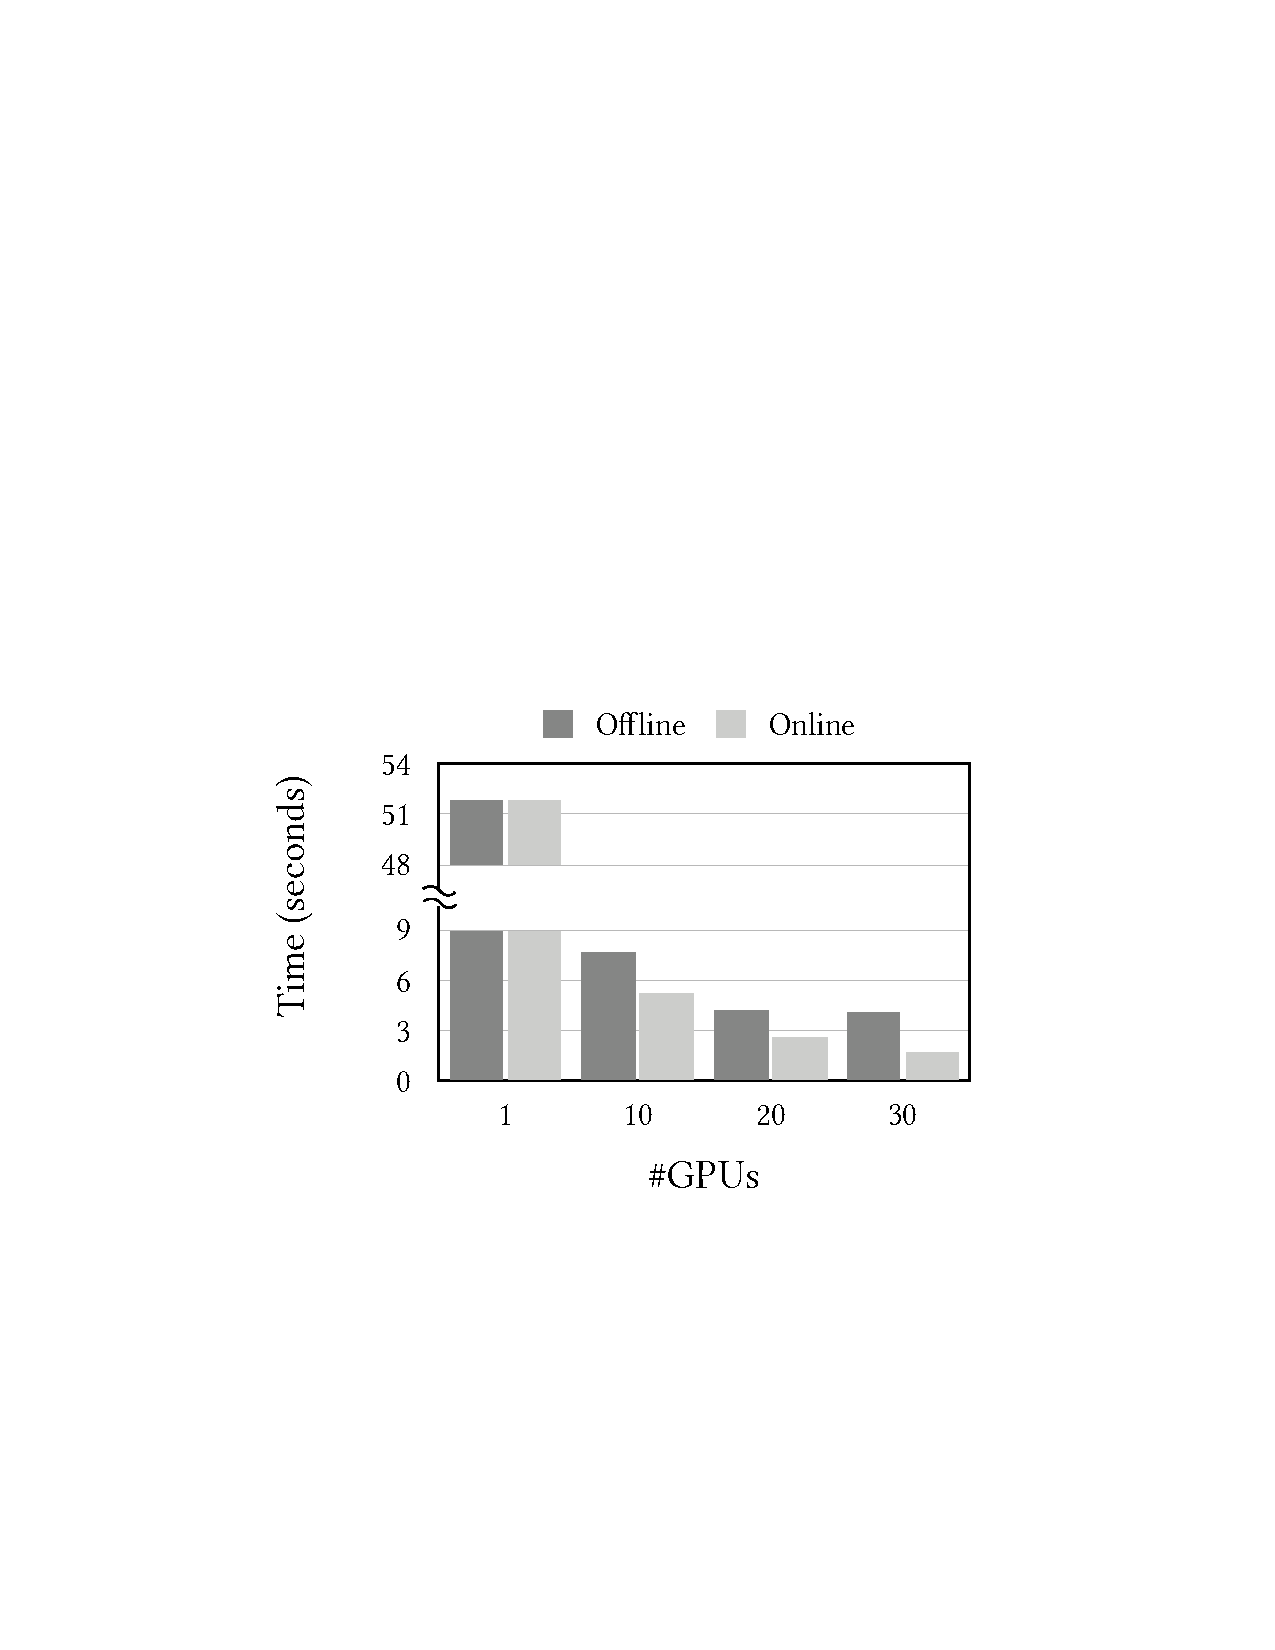
\includegraphics[width=1.0\columnwidth]{figures/parallel.pdf}
  \vspace{-1em}
  \caption{Parallelism speeds up both offline and online profiling.  The y-axis
    shows the profiling time for 1-second video.}
  \label{fig:parallel}
  \vspace{-0.5em}
\end{figure}

\para{Parallelism reduces the profiling time (\autoref{fig:parallel})}. Because
evaluating each individual configuration is independent of other configurations,
we parallelize the profiling task by assigning configurations to GPUs.
$(i)$~Our offline profiling assigns configurations randomly.  With the increased
number of GPUs, the overhead reduces from 52X to 4X with 30 GPUs.  $(ii)$~Our
online profiling assigns configurations based on the processing times collected
during offline.  \sysname{} uses LFS~\cite{karger2010scheduling} to minimize the
makespan and reduces the overhead to 1.75X with 30 GPUs (29$\times$ gain).

\para{Sampling techniques speed up online profiling
  (\autoref{fig:online-tricks}).}  Before we evaluate the speed up, we validate
\textit{model drift} with real-world data. When using the profile trained in an
office environment, the application should use a configuration of 1280x720,
\SI{30}{FPS} and 20 quantization to meet an \SI{11}{Mbps} goal. We test it
against a home environment; but at about t=100s, the camera points out of the
window to detect objects on the street. Because of the scene change, the
configuration fails to predict bandwidth, as illustrated in
\autoref{fig:offline}.

To correct the profile, if we continuously run the profiling online and update
the profile, the application will choose the right configuration to meet the
bandwidth limit.  \autoref{fig:online} shows the bandwidth prediction when we
continuously profile with the past 30 seconds of video. At time t=120s, the new
prediction corrects the drift. The downside of continuous profiling, as
discussed earlier, is the cost: 52X overhead with 1 GPU\@. In addition to
parallelism, \sysname{} uses sampling techniques for online profiling
(improvements in \autoref{tab:online}):

(i) Partial data. Instead of using all the past data, we run profiling with only
a fraction of the raw data.  \autoref{fig:online-partial} shows the bandwidth
consumption if the profiling uses only 10 seconds of data out of the past 30
seconds. In this way, although the profile may be less accurate (the
mis-prediction at t=80-100s), and there is a delay in reacting to data change
(the mis-prediction is corrected after t=125s), we save the online profiling by
3$\times$ (from 52X to 17X).

(ii) Partial configurations. If we use the past profile as a reference and only
measure a subset of $\mathbb{P}$, the savings can be substantial. A full
profiling is only triggered if there is a significant
difference. \autoref{fig:online-trigger} shows the bandwidth prediction if we
evaluate 5 configurations continuously and trigger a full profiling when the
bandwidth estimation is off by \SI{1}{Mbps} or the accuracy is off by 10\%.  For
our test data, this scheme is enough to correct model drifts by predicting an
accurate bandwidth usage (compare \autoref{fig:online} and
\autoref{fig:online-trigger}).  The overhead reduces to 6X because we run full
profiling less often (only two full profiling). It is an 8.7$\times$ gain.

\begin{figure}
  \centering
  \begin{subfigure}[t]{0.45\columnwidth}
    \centering
    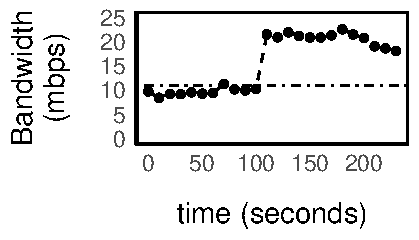
\includegraphics[width=\textwidth]{figures/online1.pdf}
    \caption{Offline only}
    \label{fig:offline}
  \end{subfigure}
  \hfill
  \begin{subfigure}[t]{0.45\columnwidth}
    \centering
    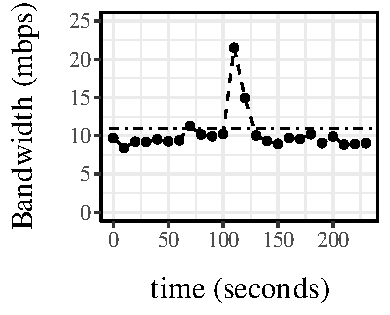
\includegraphics[width=\textwidth]{figures/online2.pdf}
    \caption{Online (continuous)}
    \label{fig:online}
  \end{subfigure}
  \\
  \vspace{0.5em}
  \begin{subfigure}[t]{0.45\columnwidth}
    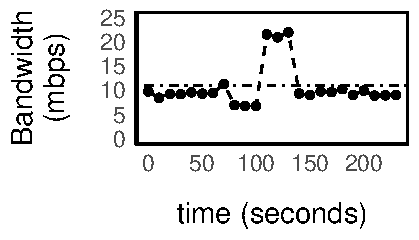
\includegraphics[width=\textwidth]{figures/online3.pdf}
    \caption{Partial data}
    \label{fig:online-partial}
  \end{subfigure}
  \hfill
  \begin{subfigure}[t]{0.45\columnwidth}
    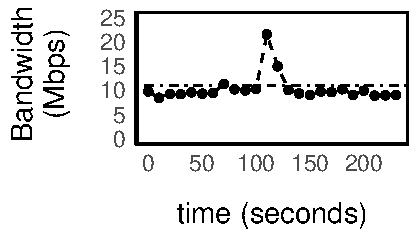
\includegraphics[width=\textwidth]{figures/online4.pdf}
    \caption{Partial configurations}
    \label{fig:online-trigger}
  \end{subfigure}
  \caption{The horizontal reference line is the target bandwidth
    (\SI{11}{Mbps}). (1) Online profiling is necessary to handle model drift
    ((a) vs.\,(b-d)). (2) Sampling techniques---partial data (c) and partial
    configurations (d)---can correct model drift with less profiling overhead
    (see \autoref{tab:online}), compared to continuous (b).  We omit accuracy
    predictions since in all schemes \sysname{} finds configurations that
    achieve similarly high accuracy (\textasciitilde 90\%).  }
  \label{fig:online-tricks}
  \vspace{-0.5em}
\end{figure}

%% Offline: 0
%% Online: 1 frame (1852.21 GPU * seconds)
%% Online (1/10)   (185.2 GPU * seconds)
%% Trigger         ( GPU * seconds)

Note that these techniques---parallelization, sampling data, and sampling
configurations---can be combined to further reduce the profiling overhead. For
example, scheduling 5 GPUs running 5 configurations continuously to check for
model drift will reduce the overhead to 1X\@. In practice, the amount of
resources to use depends on the budget and the importance of the job. \sysname{}
currently requires developers to configure the application with proper online
profiling techniques.

%% Note that it is not always needed to do online profiling. PD's test data
%% doesn't exhibit model drift.  Nor is online profiling always
%% expensive. Processing TK over all configurations.

\begin{table}[t]
  \small
  \centering
  \begin{tabular}{c c c}
    \toprule
    Online scheme & Overhead & Improvements \\
    \midrule
    Continuous & 52X & Baseline \\
    Partial data & 17X & 3$\times$\\
    Partial configurations & 6X & 8.7$\times$ \\
    \bottomrule
  \end{tabular}
  \vspace{0.5em}
  \caption{Compared to the continuous profiling baseline (52X overhead), our
    sampling techniques speed up by 3$\times$ or 8.7$\times$.}
  \label{tab:online}
  \vspace{-1em}
\end{table}

\subsection{Runtime Adaptation}
\label{sec:runtime-adaptation}

In this section, we evaluate the runtime performance by controlling bandwidth
across geo-distributed sites and compare \sysname{} with baselines including
streaming over TCP/UDP, JetStream, and video streaming. Due to limited space, we
discuss AR in depth and only present the results of PD/TK.

\para{Experiment setup.} We conduct our experiments on four geo-distributed
machines from Amazon EC2, spanning four different regions. Three (at
N.\,Virginia, Ohio, Oregon) act as worker nodes and one (at N.\,California) acts
as the analytics server. The average RTTs from the workers to the server are
\SI{65.2}{\ms}, \SI{22.2}{\ms}, and \SI{50.3}{ms}.

During the experiment, each worker transmits test data (\autoref{tab:apps}) for
about 10 mins. If the duration of the test data is less than 10 mins, it
loops. Because $B(c_{\max})$ is prohibitively large (raw videos consumes
\SI{230}{Mbps}), we use a reasonable configuration to limit the maximum rate. In
our AR experiment, $c_{\max}$ is 1600x900 resolution, \(30~\text{FPS}\) and 20
quantization; it consumes about \SI{14}{Mbps}.

Our bandwidth control scheme follows JetStream~\cite{rabkin2014aggregation}.
During the experiment, we use the Linux \texttt{tc} utility with HTB~\cite{htb,
  lartc} to control the clients' outgoing bandwidth. Each experiment involves
four phases: $(i)$~before t=200s, there is no shaping; $(ii)$~at t=200s, we
limit the bandwidth to \SI{7.5}{Mbps} for 3 minutes; $(iii)$~at t=380s, we
further decrease the bandwidth to \SI{5}{Mbps}; $(iv)$~at t=440s, we remove all
traffic shaping. For UDP, HTB doesn't emulate the packet loss or out-of-order
delivery; so we use \texttt{netem} and configure the loss probability according
to the delivery rate. Because each pair-wise connection has a different
capacity, we impose a \textit{background} bandwidth limit---\SI{25}{Mbps}---to
normalize the capacity.

We compare \sysname{} with the following baselines:

\begin{itemize}[noitemsep, nolistsep, leftmargin=*]

\item Streaming over TCP/UDP (non-adaptive). For TCP, we re-use \sysname{}
  runtime that runs over TCP but disable the adaptation. For UDP, we use
  FFmpeg~\cite{bellard2012ffmpeg} to stream video:
  RTP/UDP~\cite{schulzrinne2006rtp} for media and RTSP for
  signaling~\cite{schulzrinne1998rtsp}; as in typical video conferencing and IP
  cameras~\cite{durresi2005rtp, king2009cisco}.

\item Adaptive video streaming. We use HTTP Live Streaming (HLS) to represent
  popular adaptive video streaming techniques. Our setup resembles personalized
  live streaming systems~\cite{wang2016anatomy} but uses a smaller chunk for low
  latency (1 second instead of typical 2-10 seconds).

\item JetStream with the manual policy described in \autoref{subsec:motivation}.

\item JetStream++, a modified version of JetStream that uses the profile learned
  by \sysname{}.

\end{itemize}

At runtime, \sysname{} differs from JetStream in both policy and
adaptation. JetStream++ improves over JetStream by using our Pareto-optimal
profile. \sysname{} improves the performance further with two major changes:
$(i)$~\sysname{} directly measures the delivery rate to select an appropriate
configuration to match available bandwidth while JetStream employs a
latency-based measure of capacity ratio; $(ii)$ \sysname{} has an explicit probe
phase while JetStream changes its policy immediately after capacity ratio
changes.

\begin{figure}[t]
  \begin{subfigure}[t]{\columnwidth}
    \centering
    \includegraphics[width=0.95\columnwidth]{figures/runtime_darknet-timeseries.pdf}
    \caption{Time-series plot of the runtime behaviors: throughput (top),
      showing the effect of bandwidth shaping; latency (middle) in log scale;
      and accuracy (bottom). Overlapped lines may be hard to read; we present
      the same results in \autoref{fig:ar-runtime-boxplot} for clarity.}
    \label{fig:ar-runtime-timeseries}
  \end{subfigure}
  \vspace{0.2em}
  \\
  \begin{subfigure}[t]{\columnwidth}
    \centering
    \includegraphics[width=\columnwidth]{figures/runtime_darknet-boxplot.pdf}
    \caption{Latency and accuracy during the traffic shaping
      (i.e.,~t=200s--440s).}
    \label{fig:ar-runtime-boxplot}
  \end{subfigure}
  \caption{For AR, \sysname{} simultaneously achieves low latency and high
    accuracy (accuracy has a smaller variation).}
  \label{fig:ar-runtime}
  \vspace{-0.8em}
\end{figure}

\para{Results.} \autoref{fig:ar-runtime-timeseries} shows the runtime behavior
of \sysname{} and all baselines in time series. \autoref{fig:ar-runtime-boxplot}
summarizes the latency and accuracy with box plots during bandwidth shaping
(between t=200s and t=440s).

The throughput figure (\autoref{fig:ar-runtime-timeseries}) shows the effect of
traffic shaping. During the shaping, TCP and UDP make full use of the available
bandwidth; in comparison, \sysname{}, JetStream, JetStream++, and HLS are
conservative because of adaptation (see their throughput drops). When we stop
shaping at t=440s, TCP catches up by sending all queued items as fast as
possible. JetStream also has queued items because the policy in use (with only
three rules) cannot sustain \SI{5}{Mpbs} bandwidth. \sysname{}'s throughput
increases gradually due to the explicit probing phase. HLS is the most
conservative scheme; it does not recover from degradation until t=500s.

% summary(latency)
% Time        JetStream++        JetStream            HLS
% Min.   :206.0   Min.   :  47.14   Min.   :  541.6   Min.   :3750
% 1st Qu.:264.2   1st Qu.: 331.97   1st Qu.: 1544.6   1st Qu.:4960
% Median :322.5   Median : 539.26   Median : 1732.1   Median :5438
% Mean   :322.5   Mean   : 575.11   Mean   : 3105.8   Mean   :5578
% 3rd Qu.:380.8   3rd Qu.: 771.06   3rd Qu.: 1951.0   3rd Qu.:6270
% Max.   :439.0   Max.   :1599.51   Max.   :14245.7   Max.   :7085
% Streaming over TCP Streaming over UDP    AWStream
% Min.   :   290.8   Min.   :29.73      Min.   : 42.62
% 1st Qu.: 28042.5   1st Qu.:31.51      1st Qu.: 50.59
% Median : 54315.2   Median :33.18      Median : 79.51
% Mean   : 55596.7   Mean   :33.08      Mean   :117.72
% 3rd Qu.: 81514.5   3rd Qu.:34.90      3rd Qu.:156.22
% Max.   :117780.4   Max.   :36.29      Max.   :648.08

The latency figures (both \autoref{fig:ar-runtime-timeseries} and
\autoref{fig:ar-runtime-boxplot}) show that \sysname{} is able to maintain
sub-second latency. During the traffic shaping, TCP queues items at the sender
side for up to hundreds of seconds. In contrast, UDP always transmits as fast as
possible, leading to a consistent low latency.\footnote{FFmpeg discards packets
  that miss a deadline (\SI{33}{\ms} for \SI{30}{FPS}).} HLS's latency
fluctuates around 4-5 seconds due to chunking, buffering, and network
variations, on par with recent literature~\cite{wang2016anatomy}. Both JetStream
and JetStream++ are able to adapt during traffic shaping. With a more precise
and fine-grain policy, JetStream++ achieves a lower latency (median
\SI{539}{\ms}) in comparison to JetStream (median \SI{1732}{\ms}). Because
JetStream's runtime reacts instantaneously when the congestion condition
changes, both baselines oscillate among polices during the
experiment. \sysname{} effectively addresses the oscillation with probing and
achieves a much lower latency: median \SI{118}{\ms}, 15$\times$ improvement over
JetStream and 5$\times$ improvement over JetStream++.

% summary(accuracy)
% Time        JetStream++        JetStream           HLS
% Min.   :206.0   Min.   :0.04511   Min.   :0.5714   Min.   :0.4839
% 1st Qu.:264.2   1st Qu.:0.82776   1st Qu.:0.7854   1st Qu.:0.8414
% Median :322.5   Median :0.89079   Median :0.8401   Median :0.8795
% Mean   :322.5   Mean   :0.84882   Mean   :0.8335   Mean   :0.8684
% 3rd Qu.:380.8   3rd Qu.:0.93502   3rd Qu.:0.8952   3rd Qu.:0.9222
% Max.   :439.0   Max.   :0.98947   Max.   :0.9677   Max.   :0.9712
% Streaming over TCP Streaming over UDP     AWStream
% Min.   :0.7105     Min.   :-0.015114   Min.   :0.4516
% 1st Qu.:0.8942     1st Qu.:-0.003649   1st Qu.:0.8340
% Median :0.9261     Median : 0.003017   Median :0.8851
% Mean   :0.9181     Mean   : 0.032091   Mean   :0.8692
% 3rd Qu.:0.9545     3rd Qu.: 0.009415   3rd Qu.:0.9213
% Max.   :1.0000     Max.   : 0.925875   Max.   :0.9712

The accuracy figures (both \autoref{fig:ar-runtime-timeseries} and
\autoref{fig:ar-runtime-boxplot}) show that other than UDP, most schemes are
able to maintain high accuracy. streaming over TCP always sends data at high
fidelity, achieving the highest accuracy (median 93\%), but at a cost of high
latency. JetStream uses a manual policy that are sub-optimal in comparison to
our learned profile, so its accuracy is low (median 84\%). Using Pareto-optimal
configurations, JetStream++ is able to achieve a higher accuracy (median 89\%);
but because JetStream's runtime oscillates the policy, the accuracy has a large
variation (standard deviation 14\%). In contrast, \sysname{} chooses
configurations carefully to stay in a steady state as much as possible.  It
achieves a high accuracy of 89\% with a small variation (standard deviation
7.6\%). HLS also achieves reasonable accuracy (median 87\%) because its
adaptation of tuning resolution and encoding quality is effective in
AR. However, HLS's adaptation works poorly for PD (6\% accuracy as in
\autoref{fig:pd-runtime}).

% TK latency
% Time       Streaming over TCP Streaming over UDP    AWStream
% Min.   :210.0   Min.   : 2036      Min.   :22.29      Min.   :  48.03
% 1st Qu.:251.2   1st Qu.:11438      1st Qu.:22.42      1st Qu.: 485.08
% Median :292.5   Median :21014      Median :24.78      Median : 946.45
% Mean   :292.5   Mean   :20590      Mean   :23.85      Mean   :1145.05
% 3rd Qu.:333.8   3rd Qu.:29662      3rd Qu.:24.87      3rd Qu.:1557.20
% Max.   :375.0   Max.   :39434      Max.   :24.98      Max.   :3509.99
% > summary(accuracy)
% Time       Streaming over TCP Streaming over UDP    AWStream
% Min.   :210.0   Min.   :0.9808     Min.   :0.1097     Min.   :0.9284
% 1st Qu.:251.2   1st Qu.:0.9892     1st Qu.:0.4467     1st Qu.:0.9694
% Median :292.5   Median :0.9967     Median :0.5329     Median :0.9800
% Mean   :292.5   Mean   :0.9928     Mean   :0.5236     Mean   :0.9786
% 3rd Qu.:333.8   3rd Qu.:0.9977     3rd Qu.:0.6063     3rd Qu.:0.9883
% Max.   :375.0   Max.   :0.9991     Max.   :0.7981     Max.   :0.9991

In summary, \autoref{fig:ar-runtime} shows that \sysname{} achieves low latency
and high accuracy simultaneously. We show the results \textit{during shaping} in
a different form in \autoref{fig:intro} to discuss the trade-off between
fidelity and freshness.\footnote{We obtain \autoref{fig:intro}'s app-specific
  data by feeding PD's profile to AR. We refer to JetStream as manual policies
  in \autoref{fig:intro}.}

\begin{figure}
  \centering
  \begin{subfigure}[t]{\columnwidth}
    \captionsetup[subfigure]{aboveskip=-1em}
    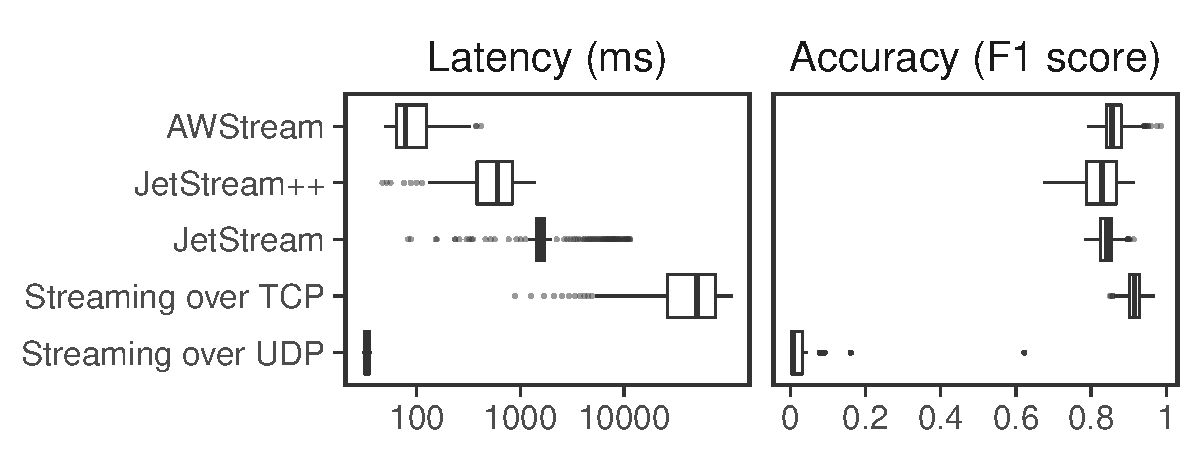
\includegraphics[width=\columnwidth]{figures/runtime_mot-boxplot.pdf}
    \begin{picture}(0,0)
      \put(-10, 80){\parbox{2cm}{\centering \caption{PD}\label{fig:pd-runtime}}}
    \end{picture}
  \end{subfigure}
  \begin{subfigure}[t]{\columnwidth}
    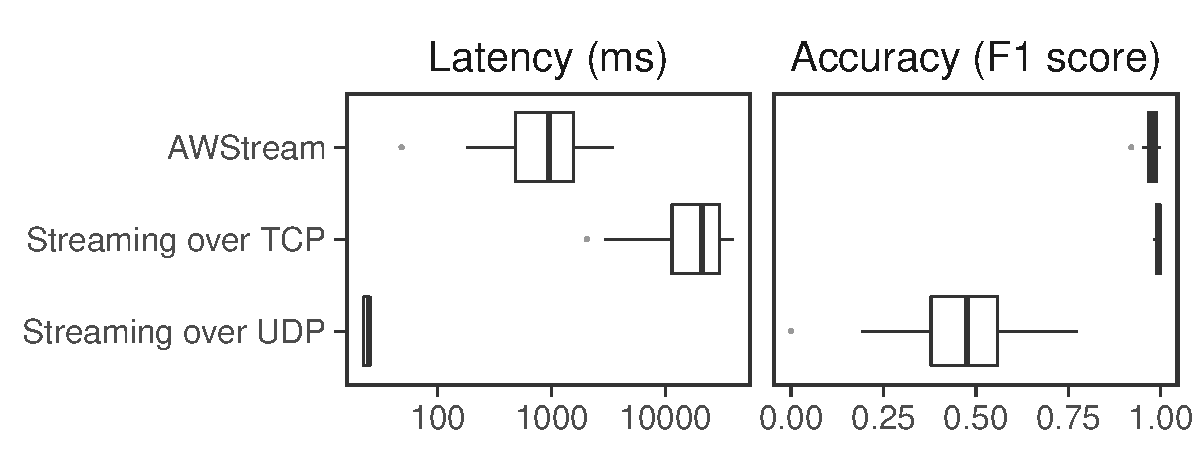
\includegraphics[width=\columnwidth]{figures/runtime_tk-boxplot.pdf}
    \begin{picture}(0,0)
      \put(-10, 60){\parbox{2cm}{\centering \caption{TK}\label{fig:tk-runtime}}}
    \end{picture}
  \end{subfigure}
  \caption{PD and TK performance summary. Box plot shows latency and accuracy
    during the traffic shaping (i.e.,~t=200s-440s).}
  \label{fig:pd-tk}
  \vspace{-1em}
\end{figure}

% \begin{figure}[t]
%   \begin{subfigure}[t]{\columnwidth}
%     \centering
%     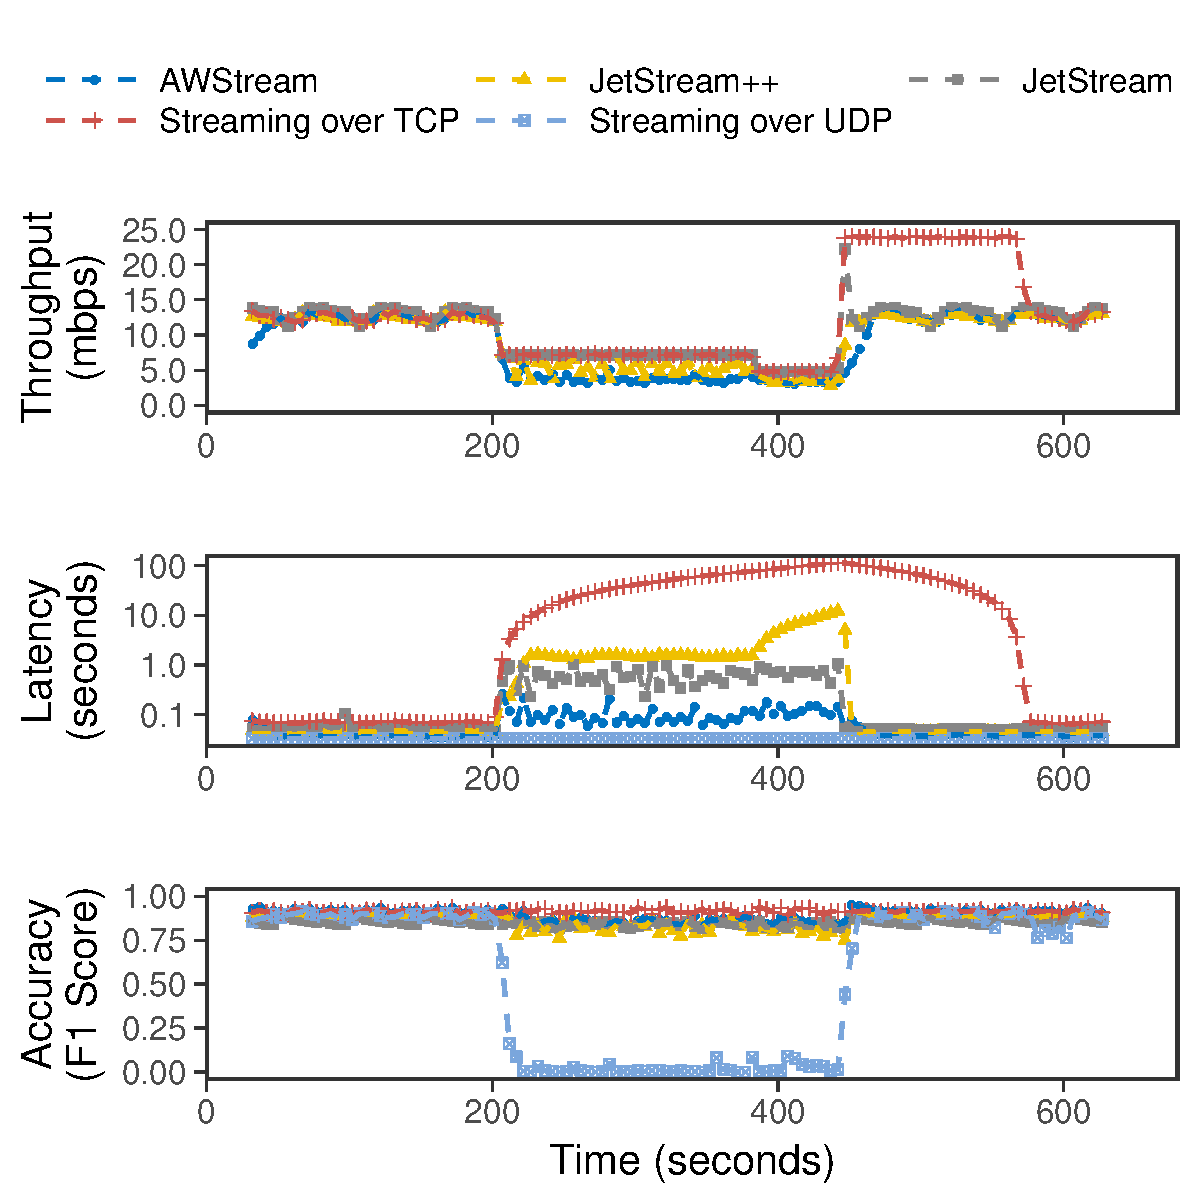
\includegraphics[width=\columnwidth]{figures/runtime_mot-timeseries.pdf}
%     \caption{PD's runtime behavior with a time-series plot: throughput (top),
%     showing the effect of bandwidth shaping; latency (middle) in log scale;
%     and accuracy (bottom).}
%     \label{fig:pd-runtime-timeseries}
%   \end{subfigure}
%   \vspace{1em}
%   \\
%   \begin{subfigure}[t]{\columnwidth}
%     \centering
%     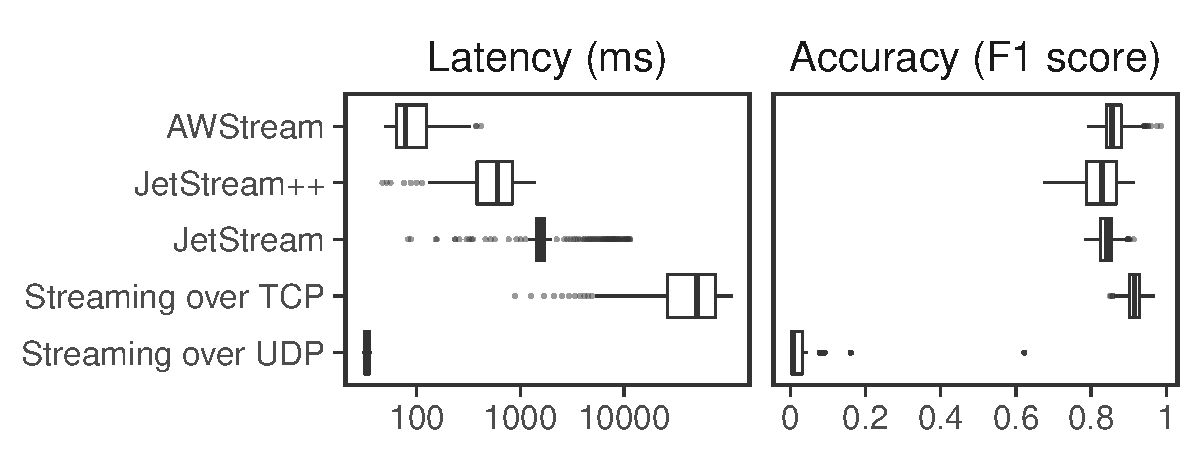
\includegraphics[width=\columnwidth]{figures/runtime_mot-boxplot.pdf}
%     \caption{PD's performance summary of latency and accuracy during the traffic
%     shaping (between t=200s and t=440s).}
%     \label{fig:pd-runtime-boxplot}
%   \end{subfigure}
%   \caption{PD runtime evaluation.}
%   \label{fig:pd-runtime}
%   \vspace{-0.5em}
% \end{figure}

% \begin{figure}[t]
%   \begin{subfigure}[t]{\columnwidth}
%     \centering
%     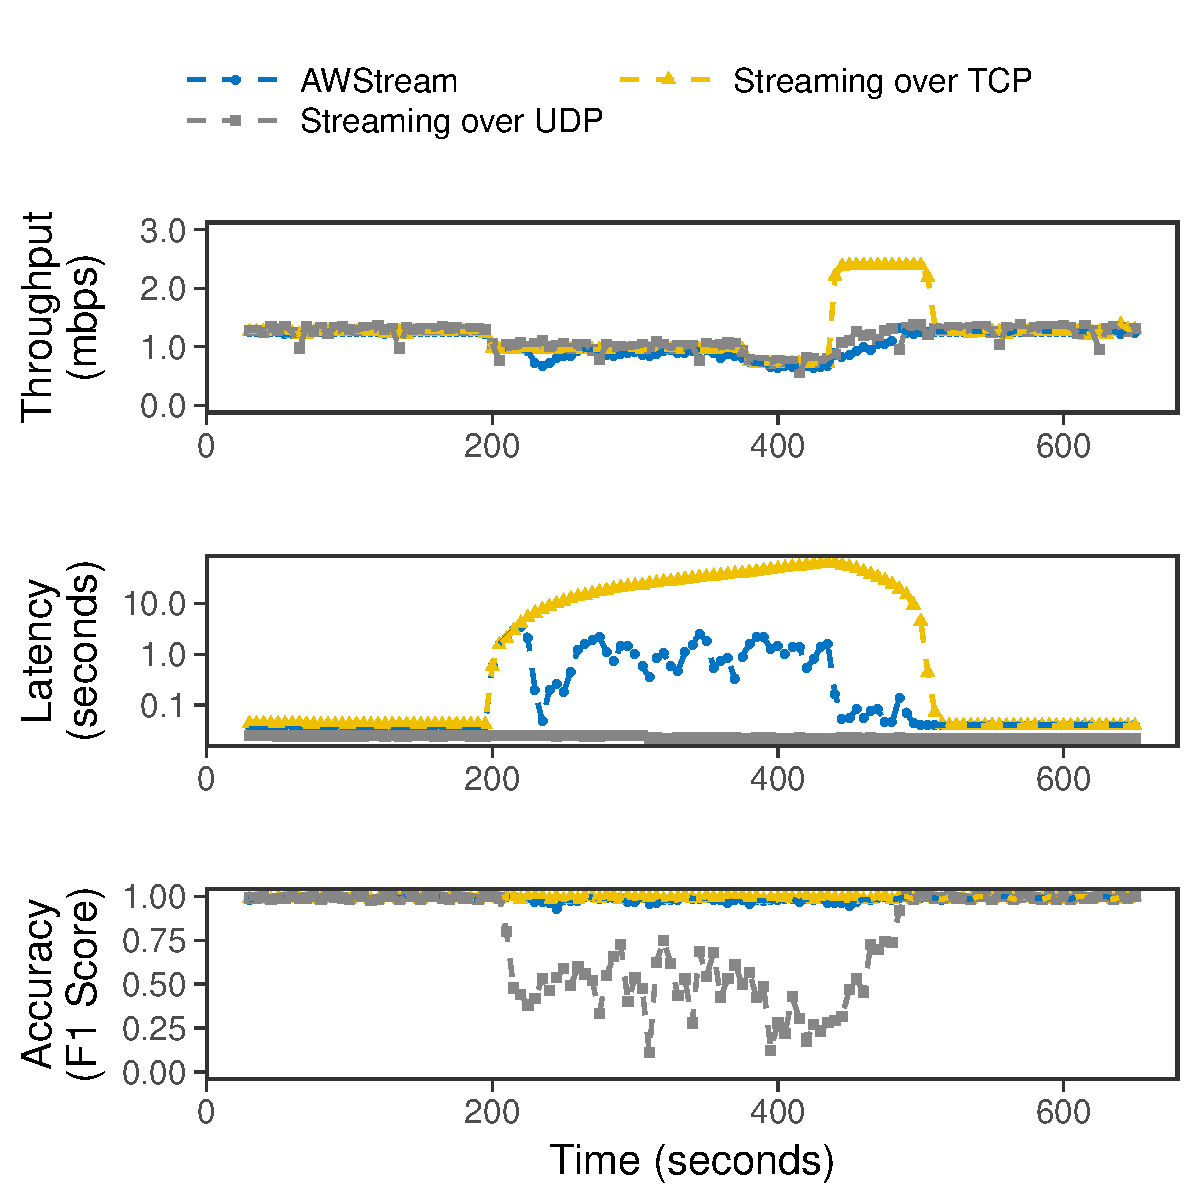
\includegraphics[width=\columnwidth]{figures/runtime_tk-timeseries.pdf}
%     \caption{TK's runtime behavior with a time-series plot: throughput (top),
%     showing the effect of bandwidth shaping; latency (middle) in log scale;
%     and accuracy (bottom).}
%     \label{fig:tk-runtime-timeseries}
%   \end{subfigure}
%   \vspace{1em}
%   \\
%   \begin{subfigure}[t]{\columnwidth}
%     \centering
%     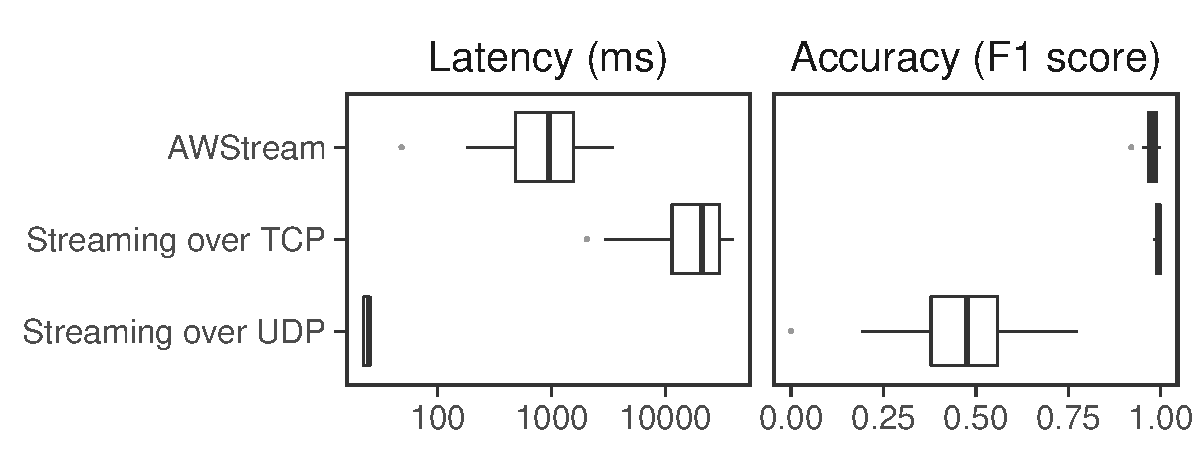
\includegraphics[width=\columnwidth]{figures/runtime_tk-boxplot.pdf}
%     \caption{TK's performance summary of latency and accuracy during the traffic
%     shaping (between t=200s and t=440s).}
%     \label{fig:tk-runtime-boxplot}
%   \end{subfigure}
%   \caption{TK runtime evaluation.}
%   \label{fig:tk-runtime}
%   \vspace{-0.5em}
% \end{figure}

\para{Pedestrian Detection.} The setup for PD is the same with AR: three clients
and one server on EC2. $c_{\max}$ is 1920x1080 resolution, \(10~\text{FPS}\) and
20 quantization; it consumes about \SI{12}{Mbps}. For PD, \sysname{} learns that
resolution is more important than frame rate. Hence it favors 1080p with 10FPS
over 900p with 30FPS. We use the same bandwidth shaping schedule and baselines
as AR. \autoref{fig:pd-runtime} shows the result and most observations about
latency/accuracy are the same as AR. HLS has a poor accuracy because it reduces
resolution and encoding quality during adaptation. \sysname{} is able to achieve
the lowest latency (\SI{78}{ms}) with small accuracy drop (86\%, 6\% drop in
comparison to TCP). In comparison to JetStream, \sysname{} improves the latency
by 20$\times$ (from \SI{1535}{ms} to \SI{78}{ms}) and accuracy by 1\% (from 84\%
to 85\%).

\para{Top-K.} For TK, we use four clients and one server because our logs are
split into four groups. $c_{\max}$ is $N=9750$ for \texttt{head} and $T=0$ for
\texttt{threshold}; it consumes about \SI{1.2}{Mbps}. Because the overall
bandwidth consumption is much smaller than video analytics, we modify the
bandwidth parameter: during t=200-380s, we limit the bandwidth to
\SI{750}{Kbps}; during t=380-440s, the bandwidth is \SI{500}{Kbps}; the
background limit is \SI{2.5}{Mpbs}. We only compared \sysname{} with streaming
over TCP and UDP. JetStream's Top-K is based on TPUT~\cite{cao2004efficient}
that targets at queries asked hourly or daily. We did not implement our Top-K
pipeline (\autoref{fig:topk}) with JetStream because video analytics suffice the
purpose of comparison. \autoref{fig:tk-runtime} shows the evaluation
results. Streaming over TCP has the highest accuracy (99.7\%) but the worst
latency (up to 40 seconds). Streaming over UDP has the lowest latency but the
worst accuracy (52\%). \sysname{} achieves low latency (1.1 seconds) and high
accuracy (98\%) simultaneously. Notice that because TK's source generates data
every second after \texttt{Window}, one object in the queue leads to one second
latency.

\vspace{0.3em}
\para{Performance with Varying Network Delays}
\vspace{0.2em}

\noindent \sysname{} targets at wide area whose key characteristic is the large
variation in latency~\cite{li2010cloudcmp}. While we have conducted experiments
using real-world setup on EC2, the latency between EC2 sites is relatively low.
To evaluate how \sysname{} performs with increased network delays, we conducted
another experiment with one pair of client and server under different network
conditions. We use \texttt{netem} to add delays, up to \SI{250}{ms} each way, so
the added RTT can be as high as \SI{500}{ms}. The delay follows a normal
distribution where the variation is 10\%, e.g.\,$250\pm 25\text{ms}$.

\begin{figure}
  \centering
  \includegraphics[width=.88\columnwidth]{figures/runtime_darknet-bench.pdf}
  \caption{\sysname{} maintains low latency and high accuracy under different
    network delay conditions.}
  \label{fig:ar-rtt}
  \vspace{-0.5em}
\end{figure}

\autoref{fig:ar-rtt} shows the runtime behavior with various added network
delays. While the latency increases with the added delay, \sysname{} mostly
manages to achieve sub-second latency for all conditions. We see a higher
variation in latency and more outliers as network delay increases, because the
congestion detection is slow when the RTT is high. In terms of accuracy, because
\sysname{} mostly stays in \texttt{Steady} state and accuracy only depends on
the level of degradation, \sysname{} achieves similar accuracy for different
network delays.

\subsection{Resource Allocation and Fairness}
\label{sec:multi-task-alloc}

\begin{figure}
  \centering
  \begin{subfigure}[t]{0.7\columnwidth}
    \centering
    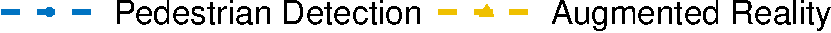
\includegraphics[width=\textwidth]{figures/multitask-legend.pdf}
  \end{subfigure}
  \\
  \vspace{0.4em}
  \begin{subfigure}[t]{0.45\columnwidth}
    \centering
    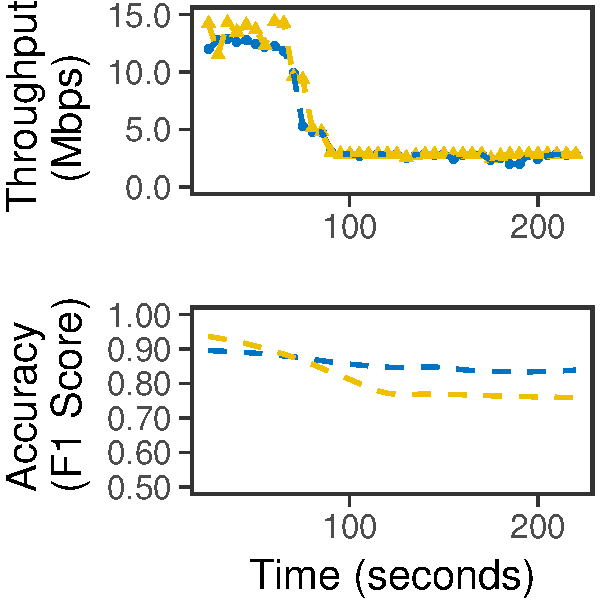
\includegraphics[width=\textwidth]{figures/multitask-left.pdf}
    \caption{Resource Fairness}
    \label{fig:eq-bw}
  \end{subfigure}
  \hfill
  \begin{subfigure}[t]{0.45\columnwidth}
    \centering
    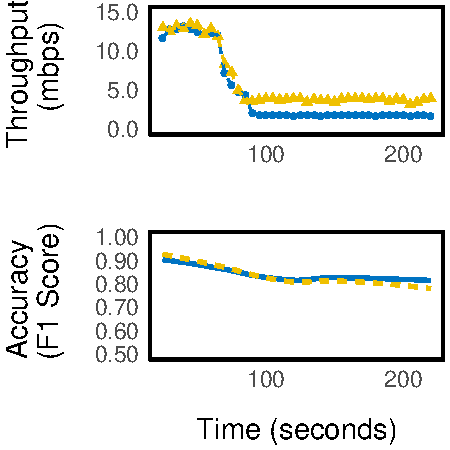
\includegraphics[width=\textwidth]{figures/multitask-right.pdf}
    \caption{Utility Fairness}
    \label{fig:eq-acc}
  \end{subfigure}
  \caption{\sysname{} allows different resource allocation schemes.}
  \label{fig:multitask}
  \vspace{-0.8em}
\end{figure}

We evaluate resource allocations with two applications. In this way, the result
also covers the case of a single application, and can generalize to more
applications.

We choose AR and PD as the example applications.  The clients and servers of
both applications are co-located so that they share the same bottleneck
link. The experiment starts with sufficient bandwidth. At t=60s, we start
traffic shaping to limit the total bandwidth to \SI{6}{Mbps}. When we allocate
resource equally between two applications (\autoref{fig:eq-bw}), each
application gets \SI{3}{Mbps}. Under this condition, PD runs with a higher
accuracy of 85\% while AR only achieves 77\%. In addition to resource fairness,
\sysname{} supports utility fairness: it chooses configurations that maximize
the minimal accuracy. In this experiment, PD receives \SI{2}{Mbps} and AR
receives \SI{4}{Mbps}; and both achieve 80\% accuracy (\autoref{fig:eq-acc}).

%%% Local Variables:
%%% mode: latex
%%% TeX-master: "../awstream"
%%% End:

%% LocalWords: TK PD runtime JetStream AR alloc YOLO dataset outliers
%% LocalWords: makespan subsec mins tcp boxplot geo HLS ffmpeg geforce
%% LocalWords: HLS PD's mis bw quantization RTSP RTP GPUs parallelization
%% LocalWords: eq netem resizes RTTs parallelize LFS UDP GTX analytics
%% LocalWords: FFmpeg GeForce HLS's JetStream's TK's tc HTB TPUT RTT